\begin{frame}[shrink=5]
    \frametitle{The FEniCS challenge!}
    Implement a famous benchmark simulating a laminar flow around 
    a cylinder. The geometry is described by
    \begin{center}
        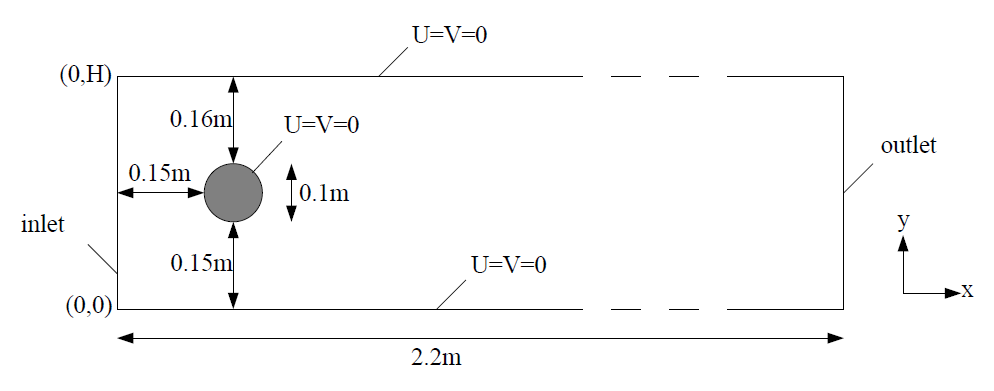
\includegraphics[width=1.0\textwidth]{png/turek_benchmark.png}
    \end{center}
    Set the  kinematic viscosity $\nu = 0.001\, \mathrm{m^2}/s$ and
    $\rho = 1.0\, \mathrm{kg}/\mathrm{m}^3$.
    A ``do-nothing'' boundary condition is assumed at the outlet.
    Defining $U_m = 1.5\,\mathrm{m}/\mathrm{s}$,
    the time-dependent inflow condition is given by
    \begin{equation*}
        U = 4 U_m y (H - y) \sin(\pi t/8)/H^2, \qquad V = 0.
    \end{equation*}
    \reference{Sch\"afer/Turek}
              {Benchmark Computations of Laminar Flow Around a
              Cylinder}
              {1996}
\end{frame}
